\chapter*{Реферат}
\addcontentsline{toc}{chapter}{Реферат} 

\begin{center}
    Общая характеристика диссертации
\end{center}

\begin{figure}
    \centering
    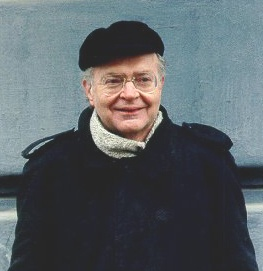
\includegraphics[width=0.6\linewidth]{images/knuth}
    \caption{Knuth}
    \label{fig:my_label2}
\end{figure}



\paragraph*{Актуальность.}

\paragraph*{Цель исследования.}
\paragraph*{Научные задачи.}

\paragraph*{Методы исследования.}


\paragraph*{Основные положения, выносимые на защиту.}
\paragraph*{Научная новизна.}
\paragraph*{Практическая значимость.}
\paragraph*{Достоверность.}
\paragraph*{Аппробация работы.}
\paragraph*{Личный вклад автора.}
\paragraph*{Публикации.}
\paragraph*{Объём и структура работы.}
Диссертация состоит из~введения,
\formbytotal{totalchapter}{глав}{ы}{}{},
заключения и
\formbytotal{totalappendix}{приложен}{ия}{ий}{}.
%% на случай ошибок оставляю исходный кусок на месте, закомментированным
%Полный объём диссертации составляет  \ref*{TotPages}~страницу
%с~\totalfigures{}~рисунками и~\totaltables{}~таблицами. Список литературы
%содержит \total{citenum}~наименований.
%
Полный объём диссертации составляет
\formbytotal{TotPages}{страниц}{у}{ы}{}, включая
\formbytotal{totalcount@figure}{рисун}{ок}{ка}{ков} и
\formbytotal{totalcount@table}{таблиц}{у}{ы}{}.
Список литературы содержит
\formbytotal{citenum}{наименован}{ие}{ия}{ий}.


\newpage
\section*{Основное содержание работы}




%\section*{Список публикаций}
%%
%% Список публикаций
%%
\ifdefmacro{\microtypesetup}{\microtypesetup{protrusion=false}}{} % не рекомендуется применять пакет микротипографики к автоматически генерируемому списку литературы
\urlstyle{rm}                               % ссылки URL обычным шрифтом
% Реализация пакетом biblatex через движок biber
% Цитирования.
%  * Порядок перечисления определяет порядок в библиографии (только внутри подраздела, если `\insertbiblioauthorgrouped`).
%  * Если не соблюдать порядок "как для \printbibliography", нумерация в `\insertbiblioauthor` будет кривой.
%  * Если цитировать каждый источник отдельной командой --- найти некоторые ошибки будет проще.
%
%% authorvak
\nocite{vakbib1}%
\nocite{vakbib2}%
%
%% authorwos
\nocite{wosbib1}%
%
%% authorscopus
\nocite{scbib1}%
%
%% authorpathent
\nocite{patbib1}%
%
%% authorprogram
\nocite{progbib1}%
%
%% authorconf
\nocite{confbib1}%
\nocite{confbib2}%
%
%% authorother
\nocite{bib1}%
\nocite{bib2}%

\insertbiblioauthorgrouped

% \ifnum \totvalue{citeexternal}>0
%     \begin{refcontext}[labelprefix=A]
%         \ifnum \value{bibgrouped}>0
%             \insertbiblioauthorgrouped    % Вывод всех работ автора, сгруппированных по источникам
%         \else
%             \insertbiblioauthor      % Вывод всех работ автора
%         \fi
%     \end{refcontext}
% \else
%     \ifnum \value{bibgrouped}>0
%         \insertbiblioauthorgrouped    % Вывод всех работ автора, сгруппированных по источникам
%     \else
%         \insertbiblioauthor      % Вывод всех работ автора
%     \fi
% \fi

%  \insertbiblioauthorimportant  % Вывод наиболее значимых работ автора (определяется в файле characteristic во второй section)
\begin{refcontext}[labelprefix={}]
    \insertbiblioexternal            % Вывод списка литературы, на которую ссылались в тексте автореферата
\end{refcontext}
% Невидимый библиографический список для подсчёта количества внешних публикаций
% Используется, чтобы убрать приставку "А" у работ автора, если в автореферате нет
% цитирований внешних источников.
\printbibliography[heading=nobibheading, section=0, env=countexternal, keyword=biblioexternal, resetnumbers=true]%


\ifdefmacro{\microtypesetup}{\microtypesetup{protrusion=true}}{}
\urlstyle{tt}                               % возвращаем установки шрифта ссылок URL